\begin{center}
	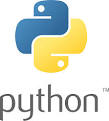
\includegraphics[width=.2\linewidth]{./IMG/python.jpg}
\end{center}
%\begin{lstlisting}
%
%import random
%import string
%import time
%
%def mkpass(size=16):
%chars = []
%chars.extend([i for i in string.ascii_letters])
%chars.extend([i for i in string.digits])
%chars.extend([i for i in '\'"!@#$%&*()-_=+[{}]~^,<.>;:/?'])
%
%passwd = ''
%
%for i in range(size):
%passwd += chars[random.randint(0,  len(chars) - 1)]
%
%random.seed = int(time.time())
%random.shuffle(chars)
%
%return passwd
%
%\end{lstlisting}

\begin{lstlisting}[style=PythonStyle, label=lst:PythonCode]
>>> a=3
>>> b=5
>>> print a+b
8
>>> print a*b
15
\end{lstlisting}

\begin{lstlisting}[style=PythonStyle, label=lst:PythonCode]
>>> for i in range(0,1000):
        print i
        i=i+1
\end{lstlisting}

\vfill\null
\pagebreak

\begin{lstlisting}[style=PythonStyle, label=lst:PythonCode]
	
%Certainly! Here is a more detailed explanation of the topics covered in the Python cheat sheet:

%Basic Syntax

%Python is a high-level, interpreted language, which means that it is executed by an interpreter rather than being compiled into machine code. This makes it easier to write and debug Python code, but also means that it may be slower than compiled languages like C or C++.
Python is case-sensitive, which means that variables and function names are treated as distinct based on whether they are written in uppercase or lowercase letters.
Indentation is used to denote blocks of code in Python. This means that statements that are part of the same block of code (e.g. the body of a for loop or an if statement) must be indented by the same number of spaces or tabs.
Lines ending in a backslash () are continued on the next line. This is often used to split long lines of code over multiple lines for readability.
%Single-line comments start with a pound sign (#). Anything following the pound sign on the same line is treated as a comment and is ignored by the interpreter.
Multi-line strings can be denoted using triple quotes (''' or """). This is often used to write long comments that span multiple lines, or to include large blocks of text in a Python program.

%Variables and Data Types

%Variables in Python are used to store values. They are assigned using the equals sign (=). For example:

%x = 10
%message = "Hello, world!"

%Python has a number of built-in data types, including integers (int), floating-point numbers (float), and strings (str). For example:

%x = 10 # integer
%y = 3.14 # floating-point number
%message = "Hello, world!" # string

%Lists and dictionaries are also commonly used data types in Python. Lists are ordered collections of items, and can contain elements of any data type. Dictionaries are unordered collections of key-value pairs. For example:

%numbers = [1, 2, 3, 4, 5] # list of integers
%names = ["Alice", "Bob", "Charlie"] # list of strings
%person = {"name": "Alice", "age": 30, "city": "New York"} # dictionary

%You can use the type() function to determine the type of a variable. For example:

%print(type(x)) # prints "<class 'int'>"
%print(type(message)) # prints "<class 'str'>"

%Operators

%Python has a number of operators that can be used to perform various operations on variables. These include:
Arithmetic operators: + (addition), - (subtraction), * (multiplication), / (division), % (modulus)
Assignment operators: = (assignment), += (add and assign), -= (subtract and assign), *= (multiply and assign), /= (divide and assign)
Comparison operators: == (equal to), != (not equal to), > (greater than), < (less than), >= (greater than or equal to), <= (less than or equal to)
The is operator is used to test whether two variables refer to the same object. For example:

%aravecchia@gmail.com
continue, please

%Certainly! Here is the remainder of the detailed explanation of the topics covered in the Python cheat sheet:

%Operators (continued)

%The is operator is used to test whether two variables refer to the same object. For example:

%x = [1, 2, 3]
y = x
z = [1, 2, 3]
%print(x is y) # prints "True"
%print(x is z) # prints "False"

%The in operator is used to test whether an element is contained in a list or dictionary. For example:

%numbers = [1, 2, 3, 4, 5]
%print(3 in numbers) # prints "True"
%print(6 in numbers) # prints "False"
%person = {"name": "Alice", "age": 30, "city": "New York"}
%print("name" in person) # prints "True"
%print("email" in person) # prints "False"

%Control Structures

%Python has several control structures that can be used to control the flow of a program. These include:
%If/elif/else statements: These are used to execute a block of code based on a condition. For example:

x = 10
if x > 5:
print("x is greater than 5")
elif x < 5:
print("x is less than 5")
else:
print("x is equal to 5")

For loops: These are used to iterate over a sequence of items. For example:

numbers = [1, 2, 3, 4, 5]
for number in numbers:
print(number)

While loops: These are used to repeat a block of code until a condition is met. For example:

x = 0
while x < 5:
print(x)
x += 1

%The range() function is often used in for loops to generate a sequence of numbers. For example:

%for i in range(5):
print(i)

%This will print the numbers 0 through 4.
The break and continue statements can be used to control the flow of a loop. The break statement is used to exit a loop prematurely, while the continue statement is used to skip the remainder of the current iteration and move on to the next one. For example:

%for i in range(10):
if i % 2 == 0:
continue
print(i)

%This will print the odd numbers from 1 to 9.

%Functions

%Python functions are defined using the def keyword. They can take arguments, and can return a value using the return keyword. For example:
%
%def add(x, y):
return x + y
result = add(10, 20)
%print(result) # prints "30"

%Python has a number of built-in functions, such as print(), len(), and range(). These functions can be called like any other function. For example:

%numbers = [1, 2, 3, 4, 5

%aravecchia@gmail.com
continue, please

%Certainly! Here is the remainder of the detailed explanation of the topics covered in the Python cheat sheet:

%Functions (continued)

%Python functions are defined using the def keyword. They can take arguments, and can return a value using the return keyword. For example:

%def add(x, y):
return x + y
result = add(10, 20)
%print(result) # prints "30"

%Python has a number of built-in functions, such as print(), len(), and range(). These functions can be called like any other function. For example:

%numbers = [1, 2, 3, 4, 5]
%print(len(numbers)) # prints "5"
%for i in range(5):
%print(i)

%You can also define your own functions in Python. For example:

%def greet(name):
%print("Hello, " + name + "!")
%greet("Alice") # prints "Hello, Alice!"
%greet("Bob") # prints "Hello, Bob!"

I hope this detailed explanation of the topics covered in the Python cheat sheet is helpful! Let me know if you have any questions or if you would like more information on any of these topics.
\end{lstlisting}